\documentclass[Review,sageapa,times]{sagej}
\renewcommand{\normalsize}{\fontsize{10}{12pt}\selectfont}
\usepackage[dvipsnames]{xcolor}

\usepackage[colorlinks,bookmarksopen,bookmarksnumbered,citecolor=CadetBlue,urlcolor=CadetBlue]{hyperref}
\usepackage{comment,moreverb,url,apacite}
\usepackage{booktabs}

\usepackage{varwidth}
\usepackage[colorinlistoftodos]{todonotes}
\makeatletter
\tikzstyle{diaanotestyle} = [
    draw=\@todonotes@currentbordercolor,
    fill=\@todonotes@currentbackgroundcolor,
    line width=0.5pt,
    inner sep = 0.8 ex,
    rounded corners=4pt,align=left,
   ]

\renewcommand{\@todonotes@drawInlineNote}{%
        {\begin{tikzpicture}[remember picture,baseline={(0,0)}]%
            \draw node[diaanotestyle,font=\@todonotes@sizecommand,anchor=base west]{%
               \begin{varwidth}[t]{5cm}
                \if@todonotes@authorgiven%
                    {\@todonotes@sizecommand \@todonotes@author:\,\@todonotes@text}%
                \else%
                    {\@todonotes@sizecommand \@todonotes@text}%
                \fi
                \end{varwidth}};%
            \end{tikzpicture}}%
       }%
\makeatother  

\usepackage{soul}
\newcommand{\mathcolorbox}[2]{\colorbox{#1}{$\displaystyle #2$}}

    
\usepackage{listings}
\definecolor{codegreen}{rgb}{0,0.6,0}
\definecolor{codegray}{rgb}{0.5,0.5,0.5}
\definecolor{backcolour}{rgb}{0.97,0.97,0.97}
\lstdefinestyle{mystyle}{
    backgroundcolor=\color{backcolour},   
    commentstyle=\color{codegreen},
    keywordstyle=\color{blue},
    %numberstyle=\tiny\color{codegray},               
    %numbers=left,                    
    %numbersep=5pt,      
    numbers=none,
    stringstyle=\color{red},
    basicstyle=\ttfamily\small,
    breakatwhitespace=false,         
    breaklines=true,                 
    captionpos=b,                    
    keepspaces=true,              
    showspaces=false,                
    showstringspaces=false,
    showtabs=false,                  
    tabsize=2,
    frameround=tttt,
    rulecolor=\color{backcolour}
}
\lstset{style=mystyle}

\newcommand\BibTeX{{\rmfamily B\kern-.05em \textsc{i\kern-.025em b}\kern-.08em
T\kern-.1667em\lower.7ex\hbox{E}\kern-.125emX}}

\def\volumeyear{2023}


\runninghead{Christensen and Buchardt}

\title{Empirical critical values for Rasch item fit statistics}

\author{Karl Bang Christensen\affilnum{1} and Ann-Sophie Buchardt\affilnum{1}}

\affiliation{\affilnum{1}Section of Biostatistics, Department of Public Health, University of Copenhagen, Denmark}

\corrauth{Karl Bang Christensen, Section of Biostatistics, Department of Public Health, University of Copenhagen, Øster Farimagsgade 5 opg. B, 1353 København K, Denmark.}

\email{kach@sund.ku.dk}

\begin{abstract}
Item fit statistics are very frequently reported in Rasch analysis. Many of them have an unknown asymptotic distribution and their interpretation rely on rules-of-thumb. 
\end{abstract}

\keywords{dichotomous Rasch model, item fit, type I error, asymptotic distribution.}

\begin{document}

%%%%%%%%%%%%
\listoftodos
%%%%%%%%%%%%


\maketitle

\section{Introduction}


\section{The \texttt{RASCHplot} R package}

The \texttt{RASCHplot} package is design to aid in visual inspection of item fit to the Rasch model. In particular, the package contains a procedure for estimating critical values for Rasch item fit statistics. In addition to making it simple and easy to create appropriate figures, the package has features that facilitate simulation of data.

The aim of the package is to provide a set of tools for both developers and end-users. 

In the following, we summarize the functionality of the R package (requiring knowledge of coding in R) and the Shiny app (a point-and-click web app with no need for coding), providing a summary in layman's terms, along with a more detailed description for the interested reader.


\subsection{Suggested workflow -- For users with coding experience}


\subsubsection{Data import}

Two numeric vectors are needed as the functions described below require a set of item parameters, $(\beta_1,\ldots,\beta_K)$, and a set of person parameters, $(\theta_1,\ldots,\theta_N)$, in two separate objects.

\subsubsection{Generating sampling distribution for a statistic of interest}

The function \texttt{simRASCHstats} implements a computational algorithm that relies on repeated random sampling to obtain a sampling distribution for an item fit statistic of interest, in particular, the outfit, infit, or item fiexperit residual. From the imported item and person parameter estimates $\hat{\boldsymbol\beta}$ and $\hat{\boldsymbol\theta}$ conditional probabilities for item responses are computed under the model \eqref{RMD} and stored in a the matrix $\boldsymbol{\hat{P}}$ defined in (\eqref{probability-matrix}). Then the \texttt{simRASCHstats} function calls the \texttt{simResps} function which, for each cell in the matrix of probabilities, generates a random number from a uniform distribution $p^{(l)}_{vi} \sim \mathcal{U}[0,1]$ and define $x^{(l)}_{vi}=1$ if $\hat{P}_{vi} > p^{(l)}_{vi}$ and $x^{(l)}_{vi}=0$ otherwise. This way we generate a data matrix  $\mathbf{x}^{(l)}$, $l=1,2,\ldots$, of item responses.
For each sample, the \texttt{simRASCHstats} function calls the wrapper function \texttt{RASCHfits}. The \texttt{RASCHfits} function calls functions implemented in other packages, see below, which estimate the parameters of a parametric IRT model using an estimation method of the users choice. Furthermore, the \texttt{simRASCHstats} calls the \texttt{RASCHstats} function which compute the item fit statistics presented above. Finally, with a user-specified number of repetitions, the function \texttt{simRASCHstats} returns an estimate of the sampling distribution for the minimum and maximum item fit statistics, $(L^{(s)})_{s=1,\ldots,B}$ and $(U^{(s)})_{s=1,\ldots,B}$, respectively. Four estimation  methods are available for the item parameter estimation through the \texttt{RASCHfits} function, namely,
\begin{itemize}
    \item PCML using the \texttt{rasch.pairwise} function from the \texttt{sirt} package \cite{sirt},
    \item CML using the \texttt{RM}  function from the \texttt{eRm} package \cite{erm},
    \item JML using the \texttt{tam.jml} function from the \texttt{TAM} package \cite{tam}, and 
    \item MML using the \texttt{tam.mml} function from the \texttt{tam.mml} package \cite{tam}.
\end{itemize} 
The default method used in the package is PCML but another method is specified via the optional argument \texttt{method.item}, which can be one of the character strings "PCML", "CML", "JML", or "MML". Two estimation methods are available for the person parameter estimation, namely WML and ML. The estimation is performed by the \texttt{IRT.mle} function from the \texttt{sirt} package. The default method is WML but ML can be specified via the optional argument \texttt{method.person}, which can be one of the character strings "WML" or "MLE".
\texttt{simRASCHstats} returns an object of class \texttt{simRASCHstats} that contains all the relevant information of the random samples for further use. We do not encourage users to extract the components directly. Instead, various methods are provided for the object such as \texttt{plot} and \texttt{print} that enable us to execute those tasks more elegantly.


\subsubsection{Visualizing empirical critical values for Rasch item fit statistics}

We can visualize the estimated sampling distribution of an item fit statistic by executing the plot method.
The \texttt{plot} function produces a density plot of the sampling distribution of an item fit statistic for a \texttt{"simRASCHstats"} object, that is, for a sampled minimum $(L^{(s)})_{s=1,\ldots,B}$ (\texttt{extreme = "min"}) or maximum $(U^{(s)})_{s=1,\ldots,B}$ (\texttt{extreme = "max"}) item fit statistic of choice. Users can choose between three different item fit statistics by specifying the argument \texttt{type}. Possible choices are \texttt{Outfit} (default), \todo[inline]{\texttt{tOutfit}}, \texttt{Infit}, \todo[inline]{\texttt{tInfit}}, and \texttt{FitResid}. Percentiles representing critical values are indicated in the figure with default values 2.5\% and 5\% for the minimum and 95\% and 97.5\% for the maximum. Users may wish to illustrate other percentiles: this can be done by specifying the argument \texttt{prob = }. 
The \texttt{plot.simRASCHstats} function is very flexible and has many arguments to allow for costumized figures. Moreover, the implementation uses the \texttt{ggplot2} package \cite{ggplot2} which gives the user all the power of the \texttt{ggplot} framework. 
To learn more, we refer to the help pages.



\subsection{The Shiny app -- a web-based application}

Shiny is an open source R package that provides an elegant and powerful web framework for building web applications using R \cite{beeley2013}. The ‘app’ can be interacted with by entering data, running functions with user-specified settings to plot figures, and downloading the resultant figures in a variety of formats.

The \texttt{RMDitemfit} Shiny app generates a sampling distribution for different Rasch item fit statistics and visualizes empirical critical values. The app is available free-of-charge (\url{https://shiny.sund.ku.dk/RMDitemfit/}) and can also be found through the \texttt{RASCHplot} package such that users can run the app locally using \texttt{RASCHplot::app("RMDitemfit")}.
The user interface of \texttt{RMDitemfit} is displayed in \autoref{fig:userinterface}. 
The sidebar panel contains input controls to select parameter estimation methods, input data, and specify the number of simulations to run. This application requires a vector of item difficulties and a vector of person parameters in two separate files. 
Users can enter their data by uploading CSV files. Once files are uploaded, the data used going forward are shown on the app landing page (the ‘Input’ tab), see \autoref{fig:inputtab}.
Subsequently, when the number of simulations is selected, users proceed to press the `Go` button to see the resultant figures. On the `Outfit` (see \autoref{fig:outfittab}), `Infit`, and `FitResid` tabs the sample distributions for the minimum and maximum outfit, infit, and item fit residuals, respectively, are shown.

\begin{figure}
    \centering
    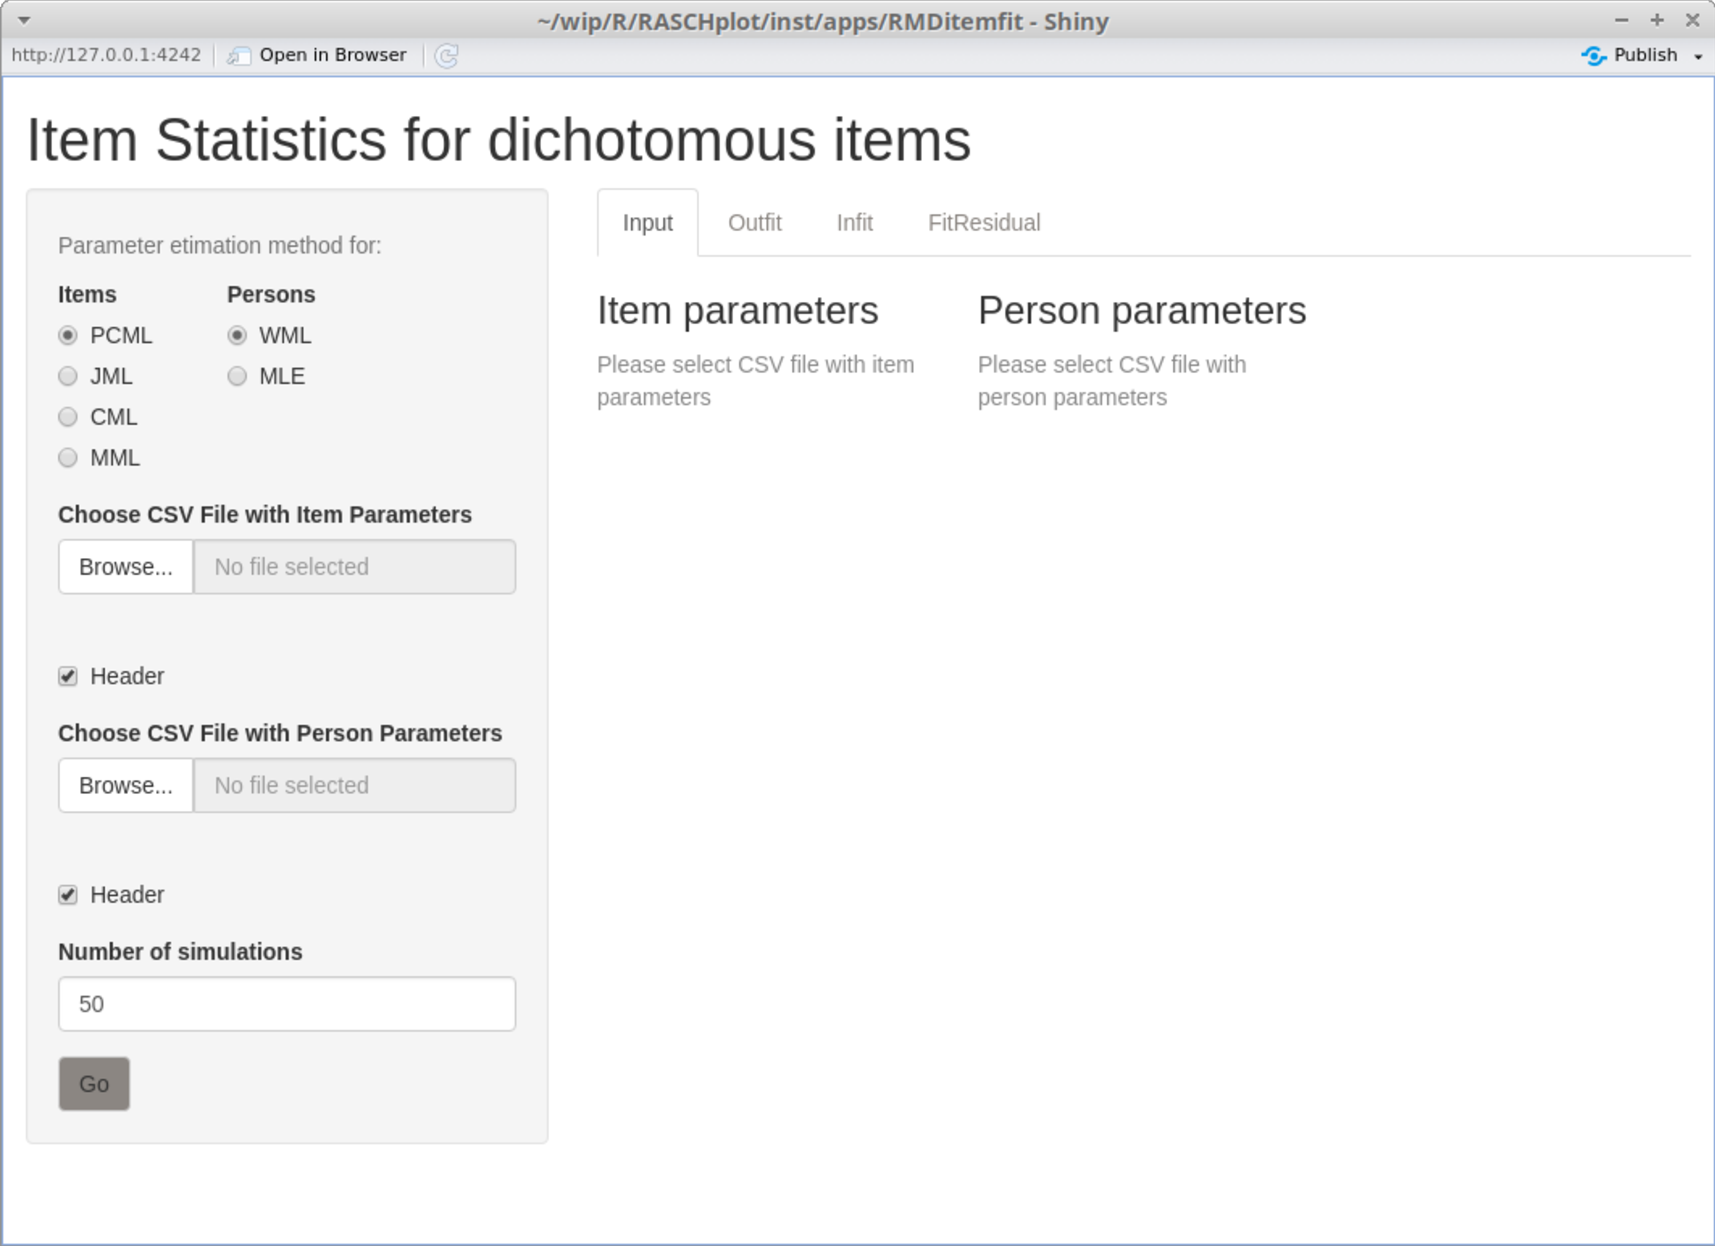
\includegraphics[width = .8\textwidth]{interface}
    \caption{Screenshot of the \texttt{RMDitemfit} Shiny app lading page.}
    \label{fig:userinterface}
\end{figure}

\begin{figure}
    \centering
    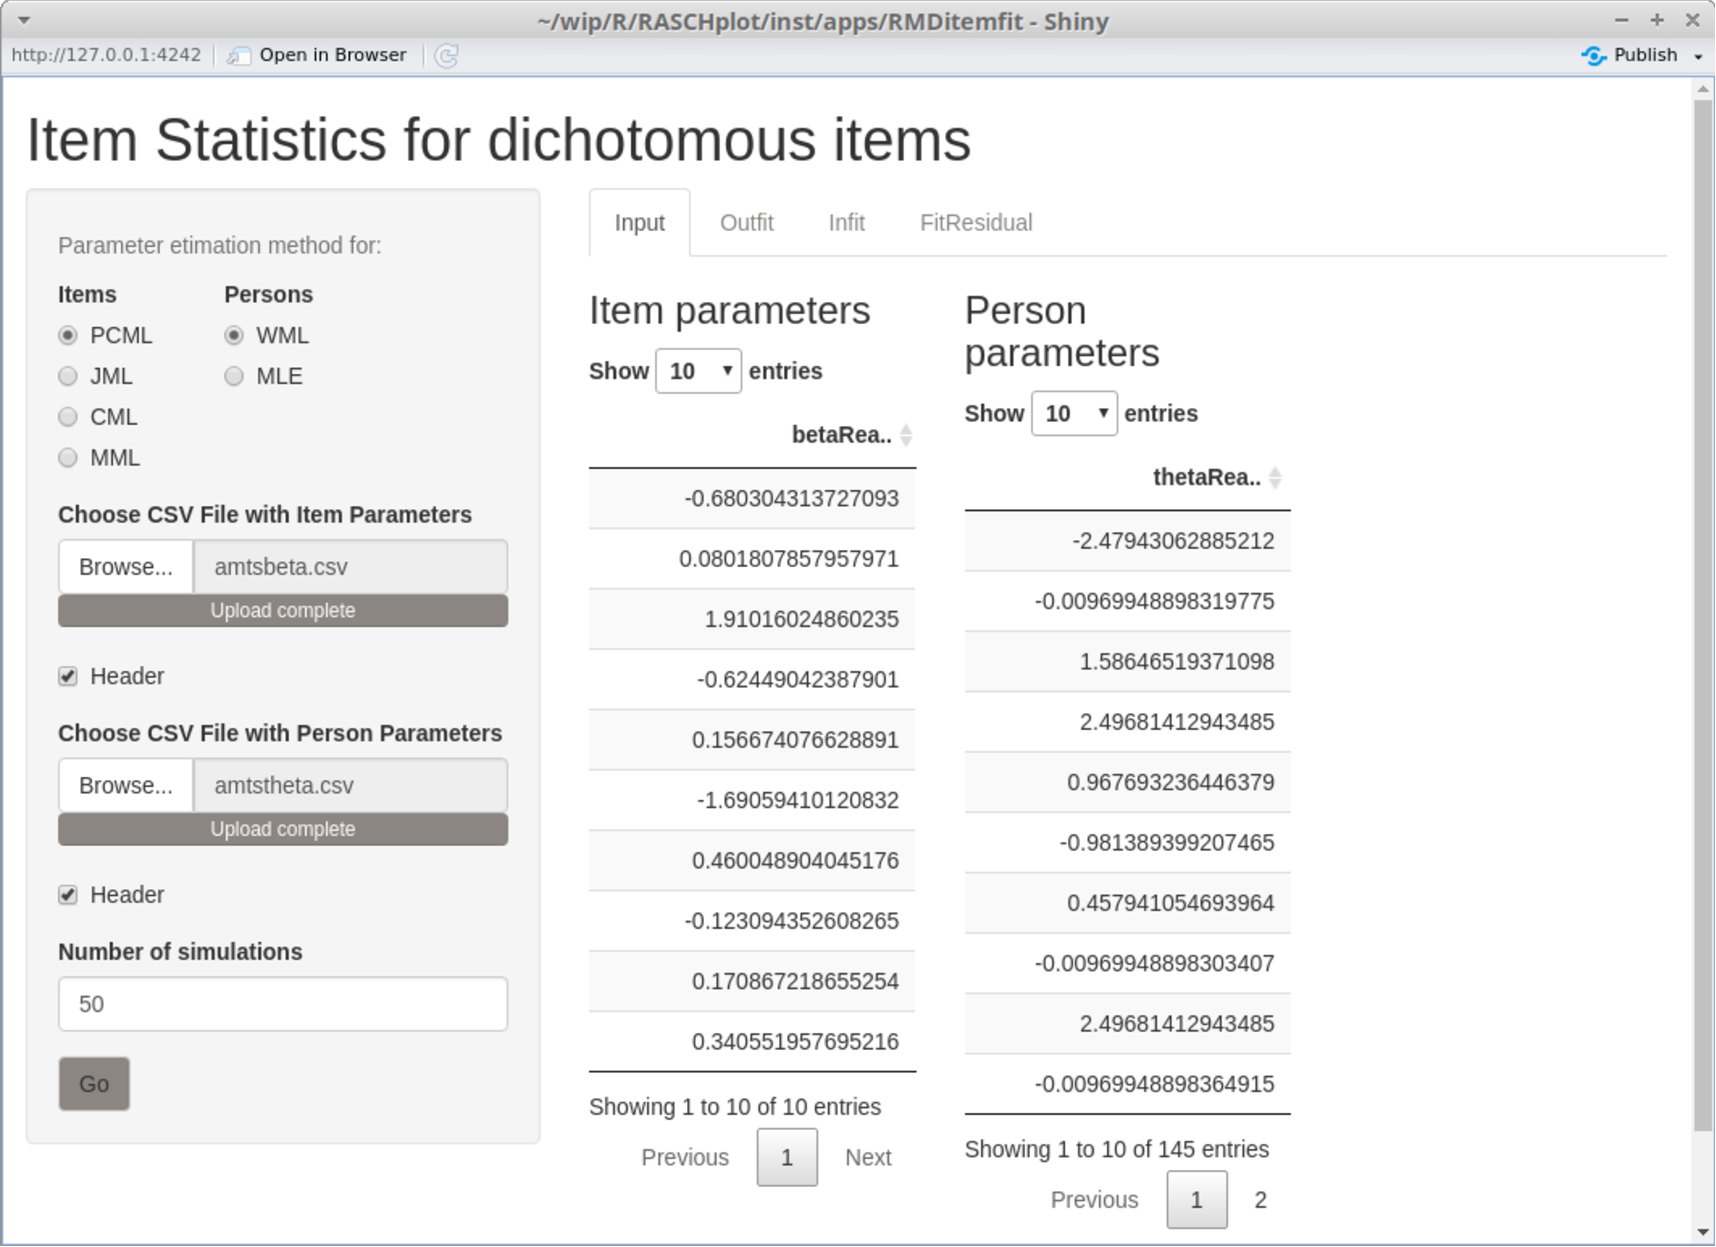
\includegraphics[width = .8\textwidth]{inputtab}
    \caption{Screenshot of the data entry page.}
    \label{fig:inputtab}
\end{figure}

\begin{figure}
    \centering
    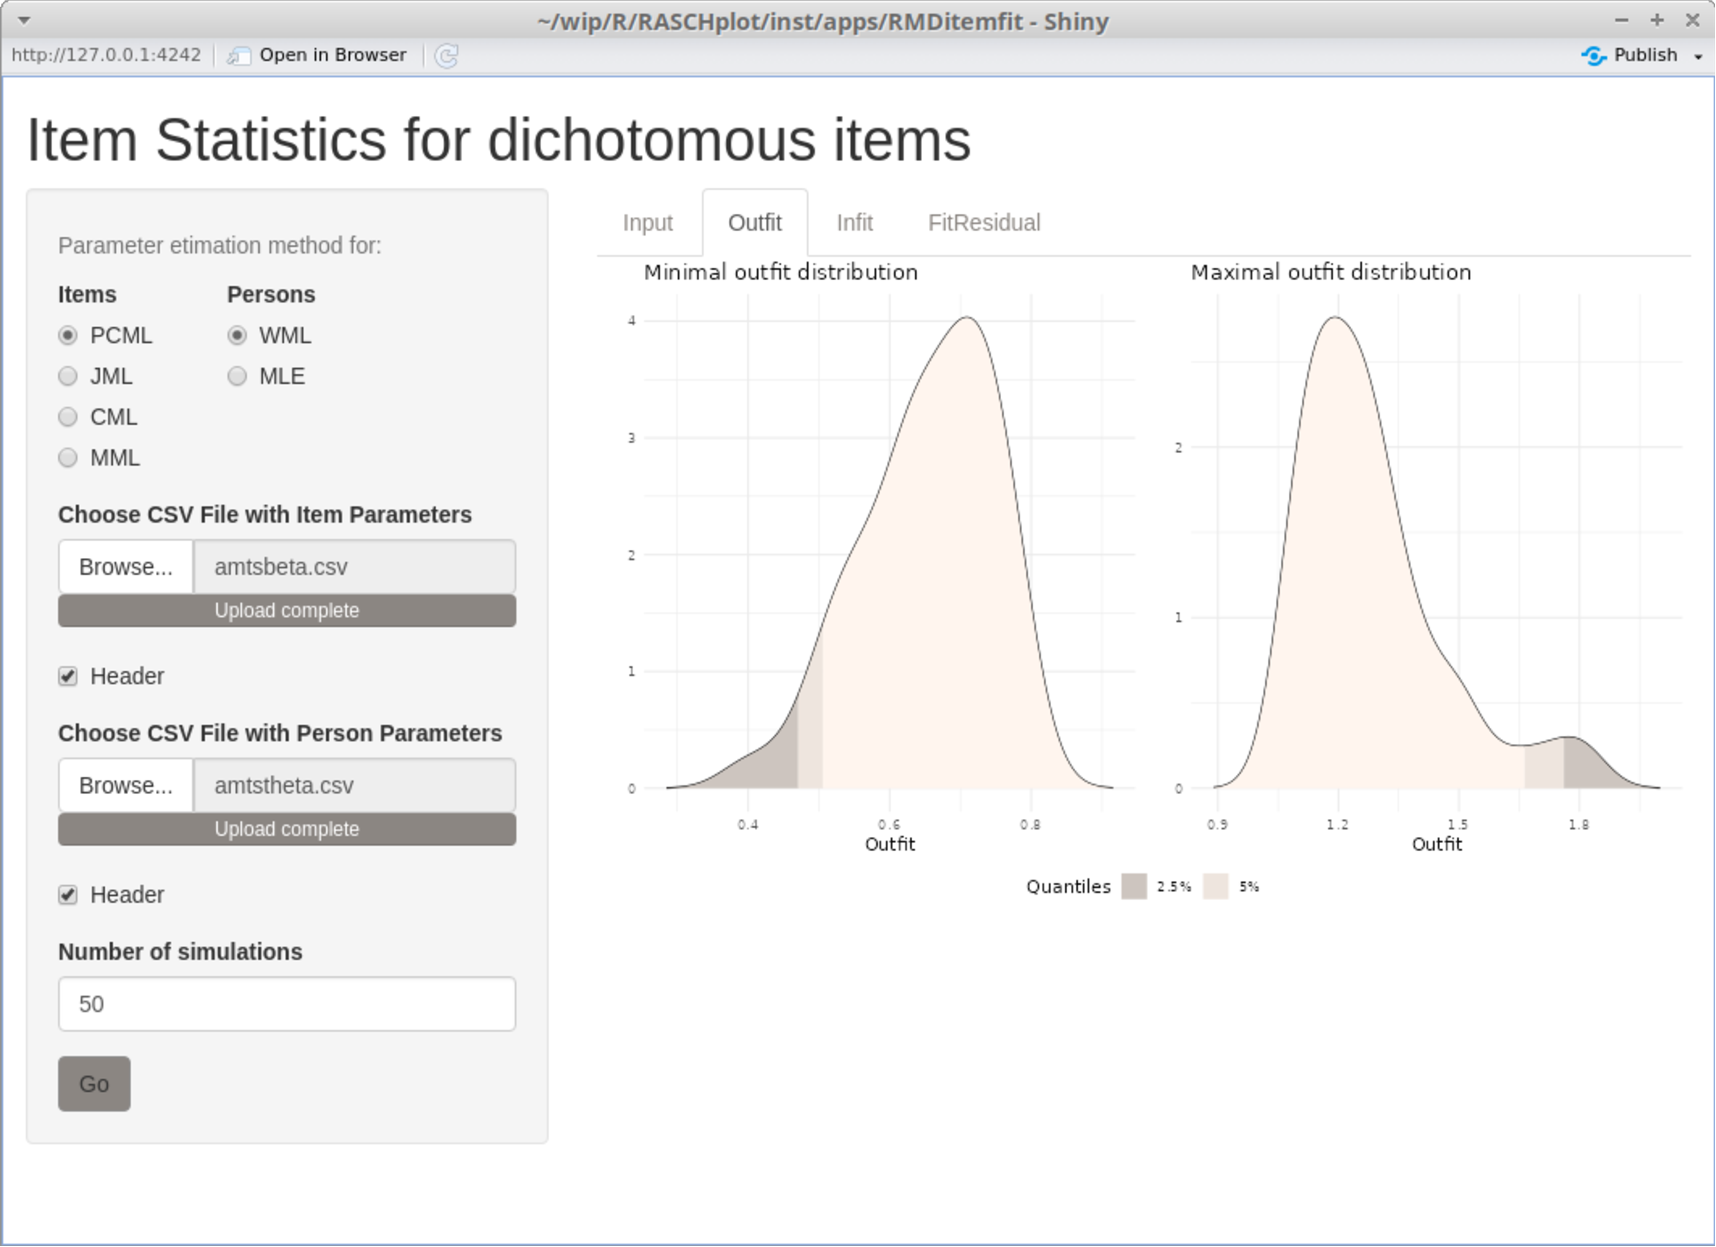
\includegraphics[width = .8\textwidth]{outfittab}
    \caption{Screenshot of the outfit item fit statistic visualisation page.}
    \label{fig:outfittab}
\end{figure}




\section{Example I: AMTS data}

This example uses the Abbreviated Mental Test Score (AMTS) \cite{hodkinson72} data  containing the responses of 197 persons to the ten questions of the AMTS. The AMTS is used to identify patients with dementia. One point is given for each correct answer, a score of 6 or less suggests that the patient has some mental impairment. 

Initial item analysis has been done in \todo{??}RUMM and resulting estimates are available at \todo{??}, see \todo{Jeg får ikke helt det samme med PCML og WML i R...?}\autoref{tab:amtsfit}. 

{\color{red}
\begin{itemize}
 \item Tabel med estimater og outfit statistics?
 \item Screen shots
\end{itemize}
}

\subsection{Details using code in R}

%The data is included as part of the \texttt{iarm} package \ref{iarm}. If the package is not installed this can be done as follows:
%\lstinputlisting[firstline=6, lastline=6, frame=single]{amtsEx.R}
%Then we include the library and load data using the \texttt{data} function.
%\lstinputlisting[firstline=7, lastline=8, frame=single]{amtsEx.R}
%Initial item analysis is done using PCML for item parameter estimation and WML for person location estimation. We use the wrapper function \texttt{RASCHfits}, which does PCML and WML estimation using the \texttt{rasch.pairwise} and \texttt{IRT.mle} functions, respectively, from the \texttt{sirt} package. If the \texttt{RASCHfits} package is not installed this can be done as follows:
%\lstinputlisting[firstline=10, lastline=11, frame=single]{amtsEx.R}
%Then data preparation and parameter estimation as follows:
%\lstinputlisting[firstline=12, lastline=23, frame=single]{amtsEx.R}

We load estimated item parameters and person locations using the \texttt{read.csv} function.

\lstinputlisting[firstline=34, lastline=35, frame=single]{amtsEx.R}

From the item parameter and person location estimates we generate a sampling distribution of the minimum and maximum outfit item fit statistic. This is done in R using the \texttt{simRASCHstats} function specifying \texttt{B = 1000} to obtain 100 random samples.

\lstinputlisting[firstline=37, lastline=40, frame=single]{amtsEx.R}

\texttt{x} is an object of class \texttt{RASCHstats} which contains all the relevant information of the repeated random sampling for further use. 
We can visualize the distribution of the sampling ditribution of the minimum outfit item fit statistic by executing the plot method:

\lstinputlisting[firstline=48, lastline=48, frame=single]{amtsEx.R}

This computes and draws a density plot with the 2.5th and 5th percentiles indicated by different colours, see the left panel of \autoref{fig:amtsOutfitMinMax}. The sampling distribution of the maximum outfit item fit statistic is visualized by specifying \texttt{extreme = "max"}, see the right panel of \autoref{fig:amtsOutfitMinMax}.

\lstinputlisting[firstline=50, lastline=50, frame=single]{amtsEx.R}

\begin{figure}
    \centering
    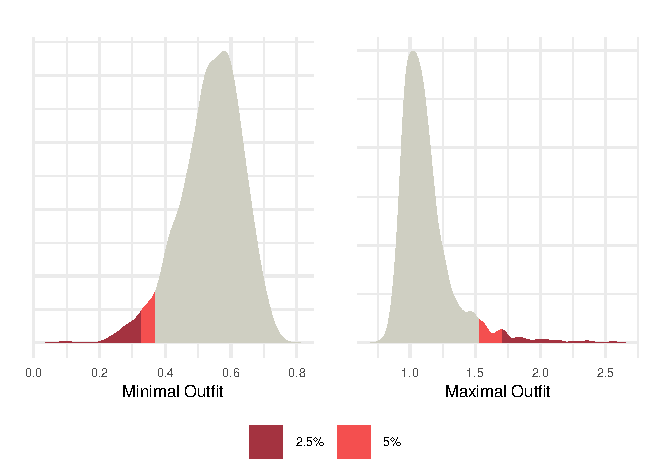
\includegraphics{amtsOutfit.pdf}
    \caption{Empirical critical values for minimum (left) and maximum (right) outfit item fit statistics for the AMTS.}
    \label{fig:amtsOutfitMinMax}
\end{figure}

\autoref{fig:amtsOutfitMinMax} shows {\color{red} ???}
\todo{Skal vi vise Infit eller Outfit?}
\todo{Skriver Infit, infit eller INFIT?}

\autoref{fig:amtsOutfitMinMax} shows {\color{red} ???}

\begin{figure}
    \centering
    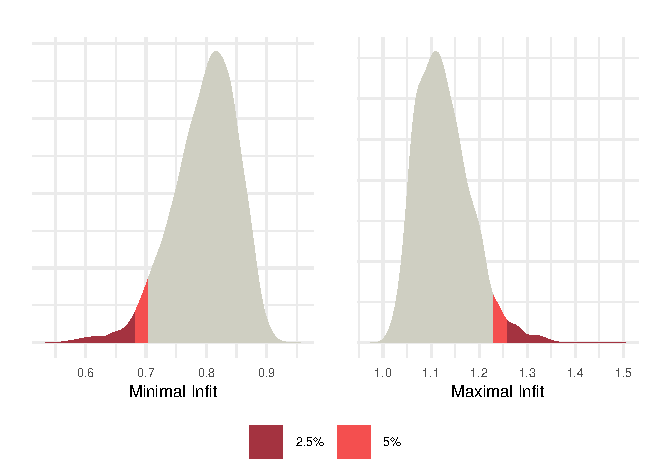
\includegraphics{amtsInfit.pdf}
    \caption{Empirical critical values for minimum (left) and maximum (right) infit item fit statistics for the AMTS.}
    \label{fig:amtsInfitMinMax}
\end{figure}

\begin{table}[b!]
    \centering
    \caption{} \label{tab:amtsfit}
    \begin{tabular}{lrrc}
    \toprule
    Item     & $\beta$ & s.e. & 95\% CI\\
    \midrule
    Address  & 2.05&0.19& 1.68 to 2.42 \\
    Age      &-0.62&0.21&-1.04 to -0.21 \\
    Countbac & 0.37&0.19& 0.00 to 0.74 \\
    Dob      &-1.72&0.25&-2.22 to -1.23 \\
    Firstww  &-0.16&0.20&-0.55 to 0.22 \\
    Monarch  & 0.17&0.19&-0.21 to 0.55 \\
    Month    & 0.37&0.19& 0.00 to 0.74 \\
    Name     &-0.62&0.21&-1.04 to -0.21 \\
    Time     & 0.05&0.19&-0.33 to 0.43 \\
    Year     & 0.13&0.19&-0.25 to 0.51 \\
    \bottomrule
    \end{tabular}
\end{table}


\end{document}